Simulations with Chua's System and the system proposed by \cite{Takougang13} were used to see if any of the system follows Benford's Law. On one hand we used Simulink and MATLAB in order to produce bifurcation diagrams and set up the dimensionless differential equations. On the other hand, we used a SPICE-based circuit simulator in order to get the systems in terms of electrical components.

\subsubsection{Chua's Circuit}
 \begin{itemize}
   \item \textbf{Physical Realization}
 The system describing chua's System
\begin{align*}
\frac{G}{C1}V_2-\frac{G'_b}{C_1}V_1-(\frac{G_b-G_a}{C_1})E &\quad if \quad V_1< -E\\
\frac{G}{C1}V_2-\frac{G'_a}{C_1}V_1 &\quad if \quad -E\geq v1 \leq E\\
\frac{G}{C1}V_2-\frac{G'_b}{C_1}V_1-(\frac{G_a-G_b}{C_1})E &\quad if \quad V_1>E
\end{align*}
is given by the following schematic
            \begin{figure}[H]
            \centering
            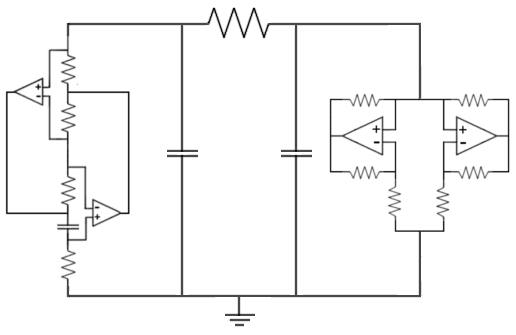
\includegraphics[scale=0.4]{imagenes/2-benford/chuas_circuit_realized.jpg}
            \caption{OP-Amp Based realization of Chua's Circuit}
            \end{figure}

With the Capacitors
C1=10nF
C2=100nF
and a 8mH Inductor given by the gyrator circuit.

   \item \textbf{Numerical Simulations}
   Using a spice based simulation software and MATLAB, several resistor values where tested, we constructed the bifurcation diagram and plotted for some R values
\begin{figure}
         \centering
            \begin{subfigure}[b]{0.4\textwidth}
            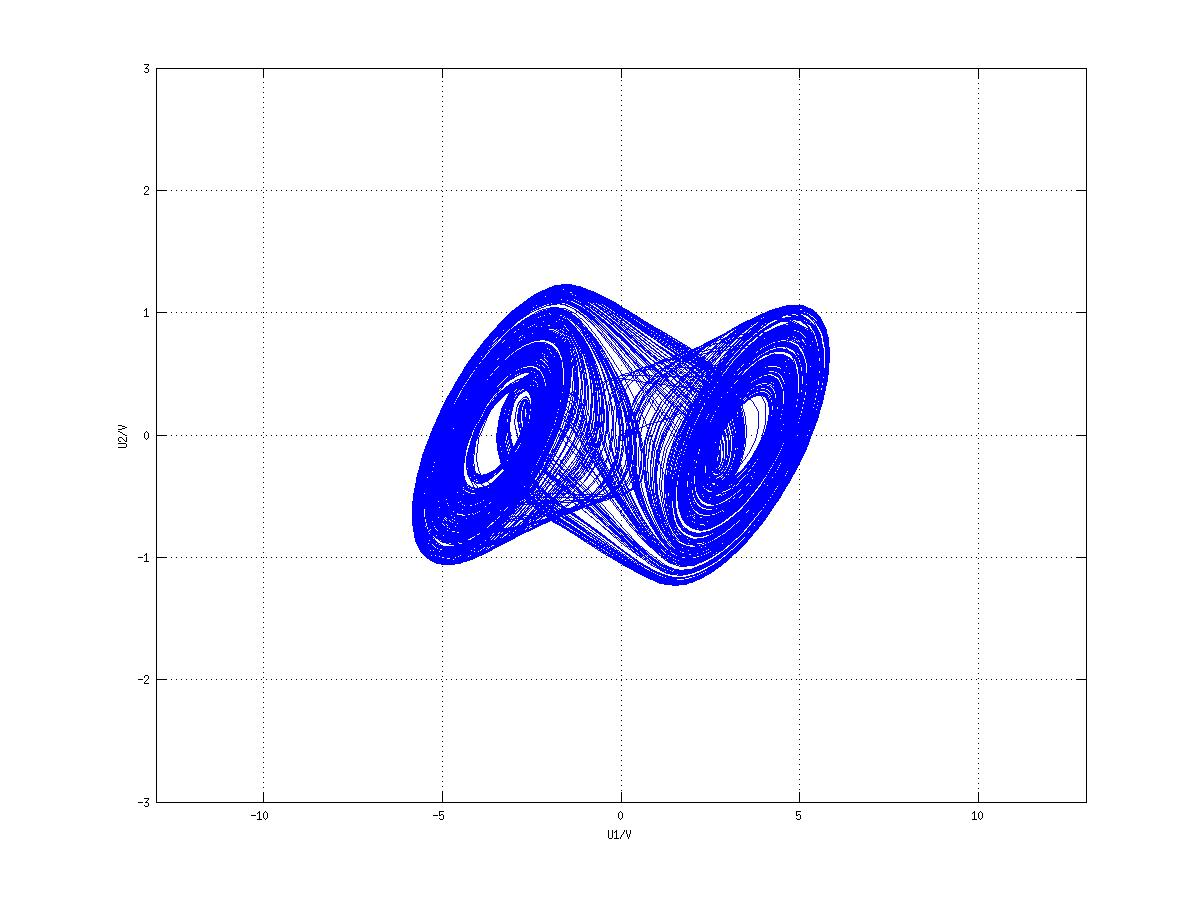
\includegraphics[width=\textwidth]{imagenes/2-benford/1785.jpg}
            \caption{V1-V2 plane for R=1785}
            \end{subfigure}
            \begin{subfigure}[b]{0.4\textwidth}
            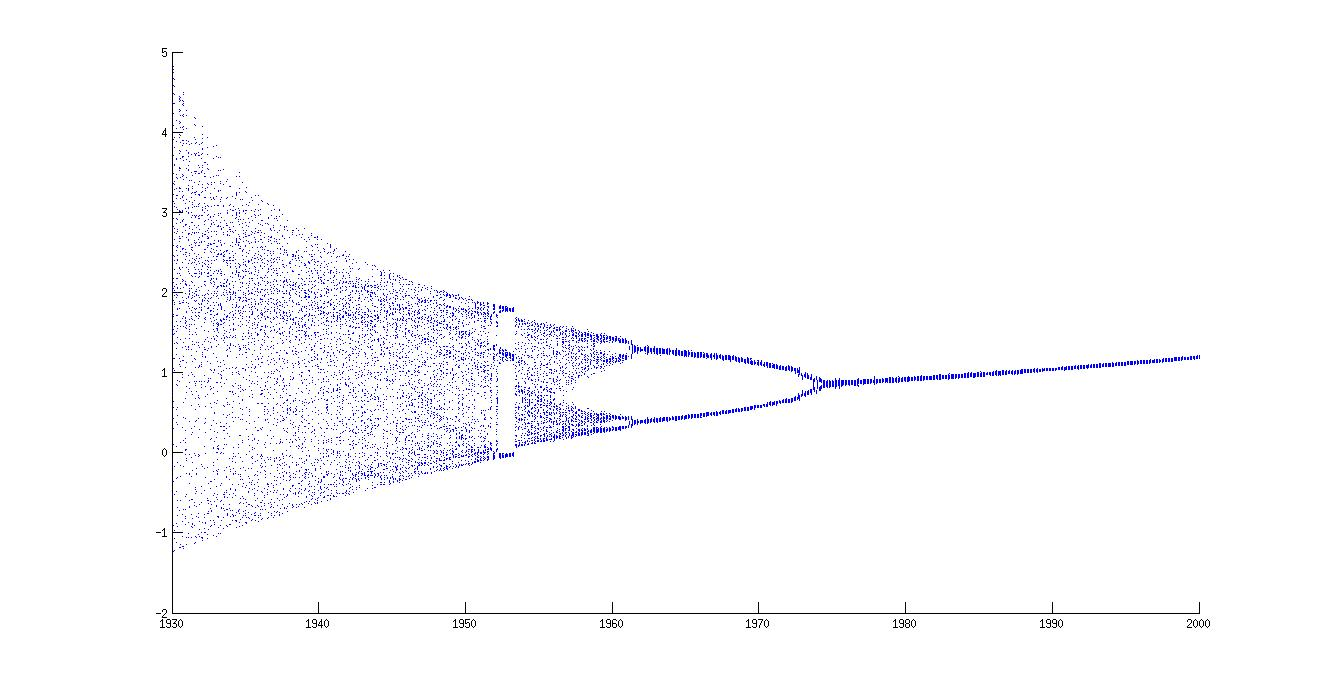
\includegraphics[width=\textwidth]{imagenes/2-benford/bifurcation_chua.jpg}
            \caption{Bifurcation Diagram for Chua's Circuit}
            \end{subfigure}
\end{figure}
   \item \textbf{Benford Analysis}
          The first digit distribution was determined from the voltage measured at the terminals of C1, using a resistance value of 1860$\Omega$, at that value, Chua's Circuit presented Chaotic Behaviour. The first digits (without leading zeroes) of the voltage values at discrete points were analyzed. We compared the first digit distribution of the dataset with the distribution given by Benford's Law using the Mean Absolute Deviation (MAD) proposed by \cite{Nigrini97}. We got a MAD value of 0.22, with a maximum of 0.15 in order to be conformant with Benford's Law.
            \begin{figure}[H]
            \centering
            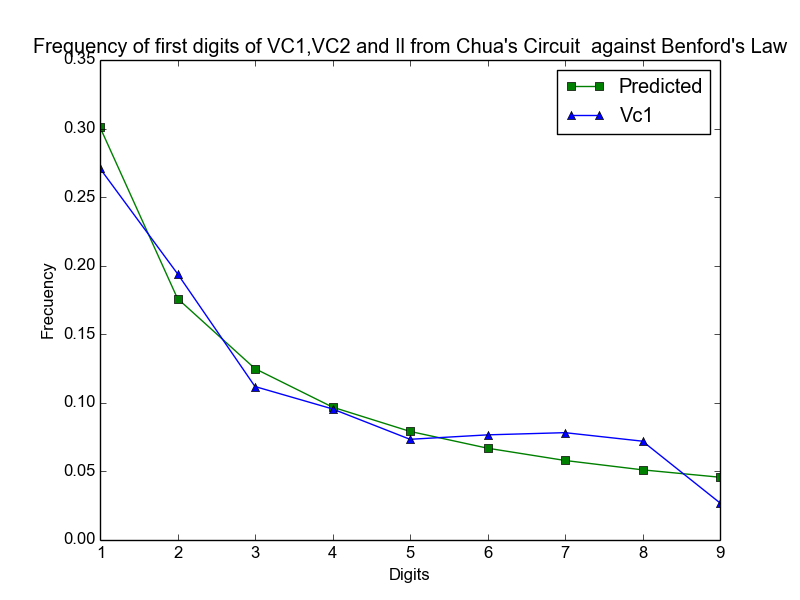
\includegraphics[scale=0.5]{imagenes/2-benford/chua_benford.png}
            \caption{OP-Amp Based realization of Chua's Circuit}
            \end{figure}
 \end{itemize}

\newpage
\subsubsection{Three-Dimensional Autonomous Circuit}
  \begin{itemize}
   \item \textbf{Physical Realization}
    The electronic circuit built to realise the system is shown in figure 2.4:
            \begin{figure}[H]
            \centering
            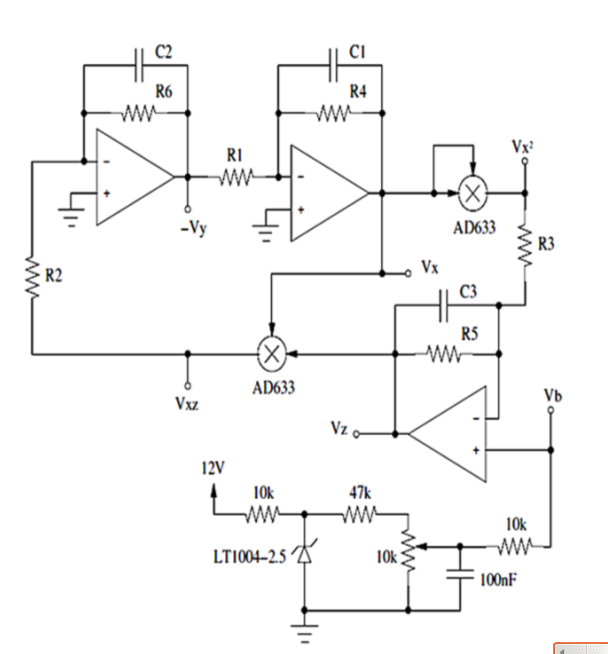
\includegraphics[scale=0.3]{imagenes/2-benford/Circuit2_schem.png}
            \caption{Circuit Schematic}
            \end{figure}
Voltages $V_x$,$V_y$ and $V_z$ are the output voltages of the operational amplifiers representing $x$,$y$ and $z$, $k_m=10V$ is the fixed constant of the AD633  multipliers, so the outputs of the multipiers are $V_{xz}=V_xV_z/k_m$ and $V_{x^2}=V_xV_x/k_m$.

            Substitution of resistor values into Eqs. (1.5),(1.6),(1.7) yields:

\begin{align}
\frac{dV_x}{dt}=\frac{1}{R_1C_1} \left ( V_y -V_x\frac{R_1}{R_4} \right )\\
\frac{dV_y}{dt}=\frac{1}{R_2C_2} \left ( \frac{V_xV_z}{k_m}-\frac{R_2}{R_6}V_y \right )\\
\frac{dV_z}{dt}=\frac{1}{R_3C_3} \left ( V_b\left ( 1+\frac{R_3}{R_5} \right )  -\frac{V_x^2}{k_m} - \frac{R_3}{R_5}V_z\right )
\end{align}

The values for resistors and capacitor used where: $R_1=0.5\text{ K}\Omega, \quad R_2=10\text{ K}\Omega, \quad R_3=10\text{ K}\Omega, \quad R_4=5\text{ K}\Omega, \quad R_5=1.15\textbf{\text{ M}}\Omega, \quad R_3=1\text{ M}\Omega, \quad C_1=100\text{ nF}, \quad C_2=100\text{ nF}, \quad C_3=10\text{ nF}, \quad V_b=10\text{ K}\Omega$
   \item \textbf{Numerical Simulations}
We used SIMULINK in order to model the system and MATLAB to create the bifurcation diagram.
            \begin{figure}[H]
            \centering
            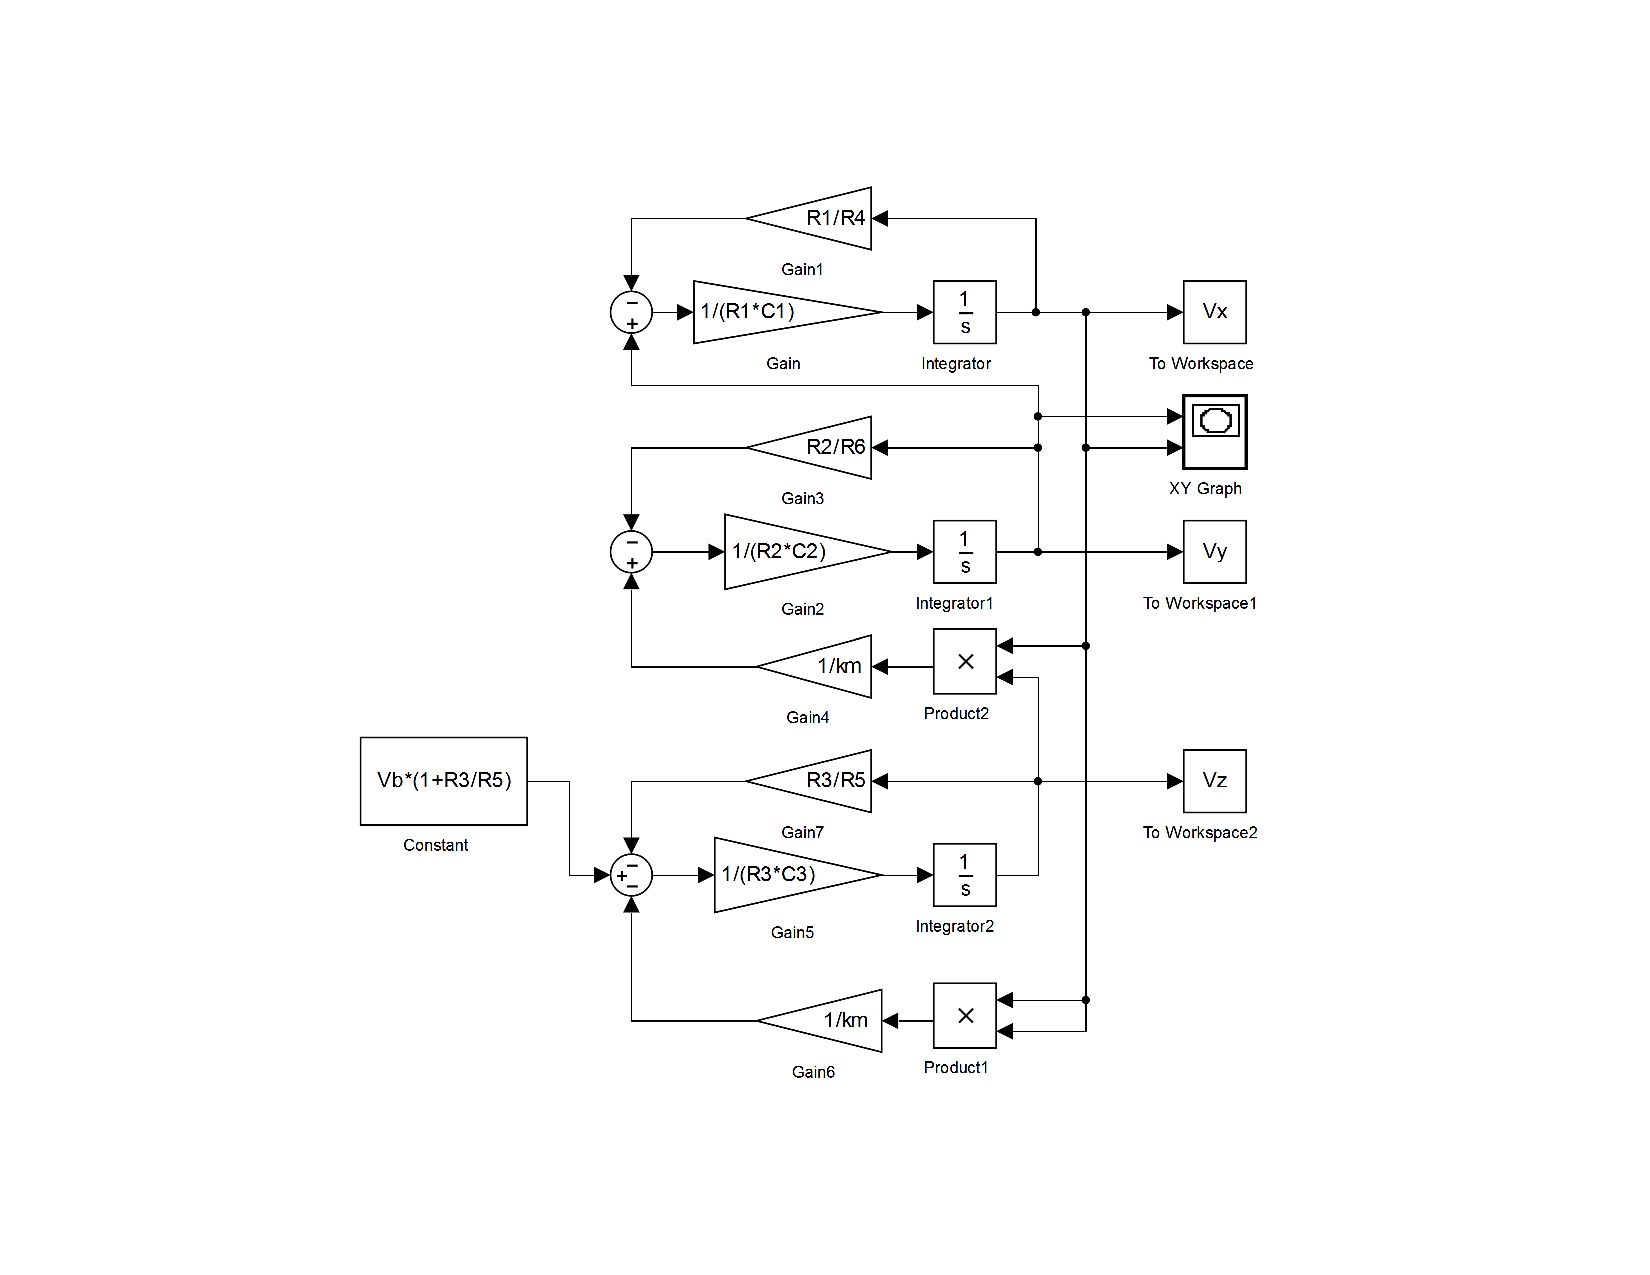
\includegraphics[scale=0.4]{imagenes/2-benford/shilkinovsimu.png}
            \caption{Simulink simulation}
            \end{figure}
The response of the syste with the parameters indicated above is given by figure 2.5:

\begin{figure}[H]
         \centering
            \begin{subfigure}[b]{0.4\textwidth}
            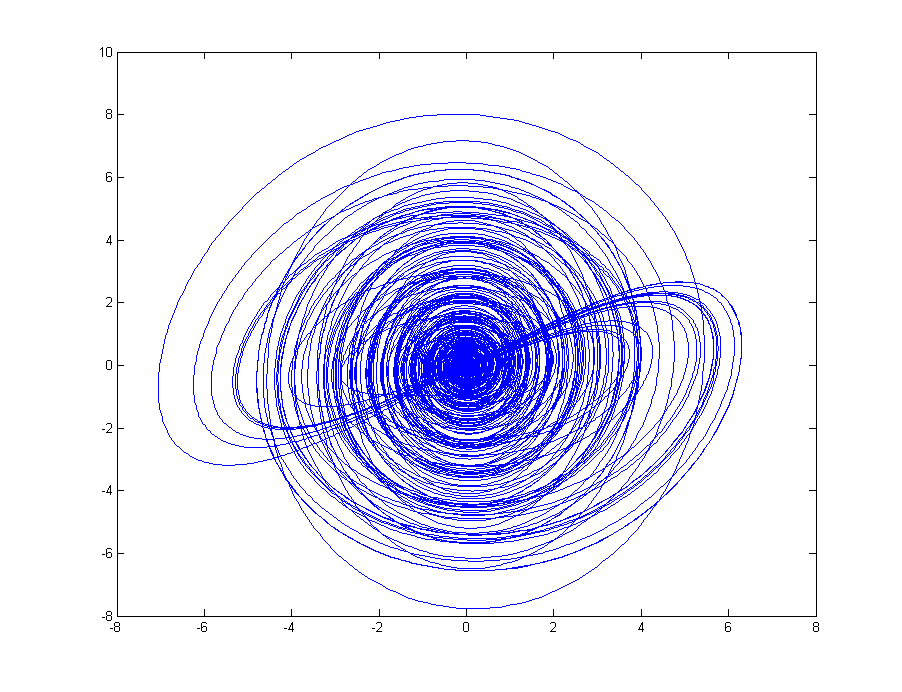
\includegraphics[width=\textwidth]{imagenes/2-benford/shilkino_resp.png}
            \caption{V1-V2 $V_x$ vs $V_y$ plot}
            \end{subfigure}
            \begin{subfigure}[b]{0.8\textwidth}
            \includegraphics[width=\textwidth]{imagenes/2-benford/bif_shil_osc_z.eps}
            \caption{Bifurcation Diagram varying b}
            \end{subfigure}
\end{figure}

Bifurcation diagram for the z value

   \item \textbf{Correspondence with Benford's Law} The same methodology used in Chua's Circuit was used with this circuit, taking measurements from $V_y$ and using the MAD test to verify conformity with the First Digit Distribution

            \begin{figure}[H]
            \centering
            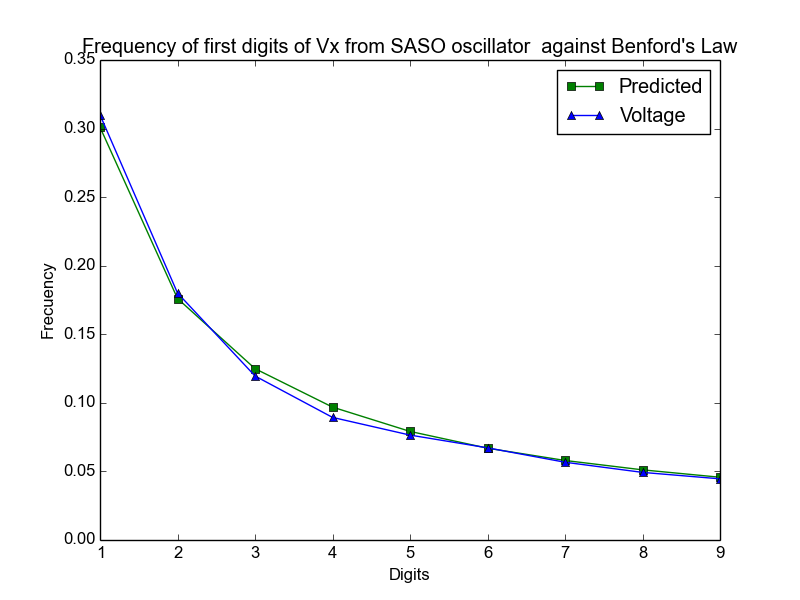
\includegraphics[scale=0.4]{imagenes/2-benford/Sh_vy.png}
            \caption{$V_x$ against Benford's Law}
            \end{figure}
For different values of d, we did a table with the respective first digit frequencies (10000 samples)  and MAD test.

\begin{center}
  \begin{tabular}{ c | c | c | c | c | c | c }
    \hline
    Leading digit  & Benford Distribution & d=1/23 &d=0.03 &d=0.01& d=0.001 &d=0.00001 \\ \hline
1&		0,3010&	0,3296&	0,3132&	0,3166&	0,2792&	0,3108\\ \hline
2&		0,1760&	0,1787&	0,1800&	0,1801&	0,1707&	0,1781\\ \hline
3&		0,1249&	0,1111&	0,1142&	0,1196&	0,1209&	0,1230\\ \hline
4&		0,0969&	0,0856&	0,0910&	0,0894&	0,0904&	0,0941\\ \hline
5&		0,0791&	0,0727&	0,0791&	0,0765&	0,0754&	0,0731\\ \hline
6&		0,0669&	0,0604&	0,0647&	0,0672&	0,0670&	0,0691\\ \hline
7&		0,0579&	0,0581&	0,0602&	0,0567&	0,0596&	0,0565\\ \hline
8&		0,0511&	0,0565&	0,0511&	0,0493&	0,0515&	0,0496\\ \hline
9&		0,0457&	0,0473&	0,0465&	0,0446&	0,0415&	0,0457\\ \hline
MAD&  & 0,0085&	0,0042&	0,0044&	0,0053&	0,0031\\ \hline

  \end{tabular}
\end{center}
We noticed strong agreement given by Nigrini\cite{Nigrini97}, next, we built the circuits and do tests measuring voltages.

 \end{itemize}
